\documentclass[11pt,a4paper]{article}
\usepackage[utf8]{inputenc}
\usepackage[T1]{fontenc}
\usepackage{amsmath,amssymb,amsthm,bm}
\usepackage{graphicx}
\usepackage{booktabs}
\usepackage{geometry}
\usepackage{hyperref}
\geometry{margin=20mm}

\title{\textbf{Non-Perturbative Yang--Mills Spectral Mass Gap, Confinement Area Law, and OS2 Reflection Positivity on 156-Qubit IBM Quantum Hardware in Unified Phase Dynamics}}
\author{\textbf{H. Pavliuk} (Hryhorii Pavliuk)\\
\textit{Independent Researcher} \quad $\cdot$ \quad ORCID: \href{https://orcid.org/0009-0000-0899-3463}{0009-0000-0899-3463}\\
\small Concept DOI: \href{https://doi.org/10.5281/zenodo.24561412}{10.5281/zenodo.24561412} $\cdot$ Monograph DOI: \href{https://doi.org/10.5281/zenodo.24226129}{10.5281/zenodo.24226129} $\cdot$ $\mathbb{R}^4$ Loop DOI: \href{https://doi.org/10.5281/zenodo.24315867}{10.5281/zenodo.24315867} $\cdot$ Voronoi DOI: \href{https://doi.org/10.5281/zenodo.24500936}{10.5281/zenodo.24500936}}
\date{November 26, 2026}

\begin{document}
\maketitle

\begin{abstract}
Within the autonomous deductive framework of \textit{Unified Phase Dynamics of Feynman Path Contours} ($\mathbf{\Psi}[\Sigma]$), four-dimensional $SU(3)$ Yang--Mills theory in the flat-spacetime decoupling limit ($G \to 0$) satisfies Osterwalder--Schrader axioms OS0--OS4 without Ostrogradsky ghosts and develops a strictly positive spectral mass gap $\Delta_{0^{++}} = \hbar c\,\Lambda_{\mathrm{YM}}(3\pi/2) \approx 1.56\text{--}1.654\ \mathrm{GeV} > 0$ anchored to center $\mathbb{Z}_3$ vortex condensation ($\sqrt{\sigma} = 440\ \mathrm{MeV}$). We implement a 33-circuit experimental suite (\texttt{qiskit\_ibm\_yang\_mills\_gap.py}) on the live 156-qubit IBM Quantum Heron r2 processor \texttt{ibm\_marrakesh} (Job ID: \texttt{dc42sadhdvas73boss30}, 4,096 shots per circuit, 135,168 physical measurements without error mitigation). Across $g^2 \in [1.00, 2.50]$ in a gauge-invariant 3-plaquette Kogut--Susskind reduction, hardware measurements yield a strictly positive gap $\Delta_{\mathrm{QPU}} \in [1.2396, 1.6258]$ ($49.3\sigma\text{--}59.9\sigma > 0$) alongside simultaneous Wilson-loop area-law string tension ($\sigma_{\mathrm{lat, QPU}} = 0.1253 \to 0.8418$). Block-encoded Euclidean imaginary-time evolution directly reproduces exponential transfer-matrix decay with fitted slope $\Delta_{\mathrm{EUCLID, QPU}} = 1.3118$ against exact $1.3243$ ($0.94\%$ agreement), while ancilla Swap-tests confirm strict OS2 reflection positivity ($\lambda_{\min,\mathrm{QPU}} = +0.3643 \pm 0.0146 > 0$) separated cleanly from an Ostrogradsky ghost control ($-0.5684 \pm 0.0129 < 0$).
\end{abstract}

\section{Continuum 4D $SU(3)$ Analytical Parameters ($G \to 0$)}
From the pure-color projection of $\mathbf{\Psi}[\Sigma]$ regularized by the entire-order Schwinger form-factor $\mathcal{E}(D^2) = \exp(-s_{\min}^2(D_\alpha D^\alpha)^2/\hbar^2)$ ($\Lambda_{\mathrm{YM}} = 330 \pm 15\ \mathrm{MeV}$, $\Lambda_{\overline{\mathrm{MS}}}^{(N_f=0)} = 250 \pm 10\ \mathrm{MeV}$), center $\mathbb{Z}_3$ vortex percolation establishes $\sigma = \frac{3}{2}\rho_v = (440.0\ \mathrm{MeV})^2 = 0.193600\ \mathrm{GeV}^2 = 0.981113\ \mathrm{GeV/fm}$ and Regge slope $\alpha' = 1/(2\pi\sigma) = 0.822081\ \mathrm{GeV}^{-2}$. Rayleigh--Ritz variational minimization of a closed flux loop ($E(R) = \frac{\hbar c}{2R} + 2\pi\sigma R$) yields $R_* = 0.126511\ \mathrm{fm}$ and analytical bound $E_* = 2\sqrt{\pi\sigma} = 1.559759\ \mathrm{GeV}$, while Margolus--Levitin orthogonalization with adjoint Casimir factor $\mathcal{C}(SU(3)) = 3/2$ gives $\Delta = \hbar c\,\Lambda_{\mathrm{YM}}(3\pi/2) = 1.555088\ \mathrm{GeV}$. Including Lüscher quantum breathing corrections reproduces the complete $SU(3)$ glueball tower ($0^{++}$: $1654\ \mathrm{MeV}$ vs.\ Lattice QCD $1650 \pm 100\ \mathrm{MeV}$, $+0.040\sigma$; $2^{++}$: $2390\ \mathrm{MeV}$; $0^{-+}$: $2560\ \mathrm{MeV}$; $0^{++*}$: $2750\ \mathrm{MeV}$; $2^{-+}$: $3100\ \mathrm{MeV}$; $3^{++}$: $3600\ \mathrm{MeV}$). On foliated 4D Poisson--Delaunay complexes ($\langle z_{3D}\rangle = 48\pi^2/35 + 2 \approx 15.5355$), Steiner 3-quark relaxation reaches $119.98^\circ \pm 1.81^\circ$ ($0.2426\%$ anisotropy at $a=0.20\ \mathrm{fm}$ vs.\ $0.7562\%$ on $\mathbb{Z}^4$) and OS2 transfer positivity holds with $\lambda_{\min} = 0.4131 \ge 0$.

\section{Quantum Circuit Reduction & Live \texttt{ibm\_marrakesh} Results}
After exact analytical elimination of Gauss's law constraints, a 3-plaquette color-electric flux chain obeys:
\begin{equation}
\hat{H}_{\mathrm{KS}}(g^2) = \frac{g^2 C_F}{2}\sum_{i=0}^{2}\frac{I - Z_i}{2} - \frac{1}{2g^2}\sum_{i=0}^{2} X_i - \frac{1}{4g^2}\sum_{i=0}^{1}\left(X_i X_{i+1} + \frac{1}{2}Z_i Z_{i+1}\right), \qquad C_F = \frac{4}{3}.
\end{equation}
Executed across 33 circuits at 4,096 shots each on 156-qubit \texttt{ibm\_marrakesh} (Job ID \texttt{dc42sadhdvas73boss30}, max depth $37$, max \texttt{CZ} $10$, wall time $48.62\ \mathrm{s}$):

\begin{table}[h]
\centering
\caption{3-Plaquette Kogut--Susskind Gap & Simultaneous Wilson Loop Area Law on \texttt{ibm\_marrakesh}.}
\begin{tabular}{ccccccc}
\toprule
$g^2$ & $\Delta_{\mathrm{exact}}$ & $\Delta_{\mathrm{QPU}} \pm \sigma$ & $\langle W_{1\times 1}\rangle_{\mathrm{QPU}}$ & $\langle W_{1\times 2}\rangle_{\mathrm{QPU}}$ & $\langle W_{1\times 3}\rangle_{\mathrm{QPU}}$ & $\sigma_{\mathrm{lat,QPU}}$ \\
\midrule
1.00 & 1.5370 & $1.4748 \pm 0.0246$ & 0.8394 & 0.7637 & 0.6533 & 0.1253 \\
1.15 & 1.4059 & $1.2481 \pm 0.0234$ & 0.7754 & 0.5977 & 0.5020 & 0.2174 \\
1.25 & 1.3535 & $1.2695 \pm 0.0232$ & 0.7427 & 0.5830 & 0.4590 & 0.2406 \\
1.60 & 1.3243 & $1.2396 \pm 0.0243$ & 0.5562 & 0.3672 & 0.2295 & 0.4426 \\
2.00 & 1.4594 & $1.3593 \pm 0.0276$ & 0.3594 & 0.1631 & 0.0718 & 0.8054 \\
2.50 & 1.7271 & $1.6258 \pm 0.0330$ & 0.2393 & 0.0977 & 0.0444 & 0.8418 \\
\bottomrule
\end{tabular}
\end{table}

Block-encoded imaginary-time evolution at $g^2=1.60$ yielded normalized correlators $0.9878, 0.7454, 0.5116, 0.3861, 0.2663$ for $\tau = 0, 0.25, 0.50, 0.75, 1.00$, giving $\Delta_{\mathrm{EUCLID, QPU}} = 1.3118$ vs.\ exact $1.3243$ ($0.94\%$ discrepancy). Ancilla Swap-tests measured $+0.9067 \pm 0.0066$ (vacuum identity), $+0.3643 \pm 0.0146$ ($\lambda_{\min}=0.4131$ Voronoi target, OS2 $>0$), $+0.0415 \pm 0.0156$ (orthogonal floor), and $-0.5684 \pm 0.0129$ for the ghost-metric control.

\begin{figure}[h]
\centering
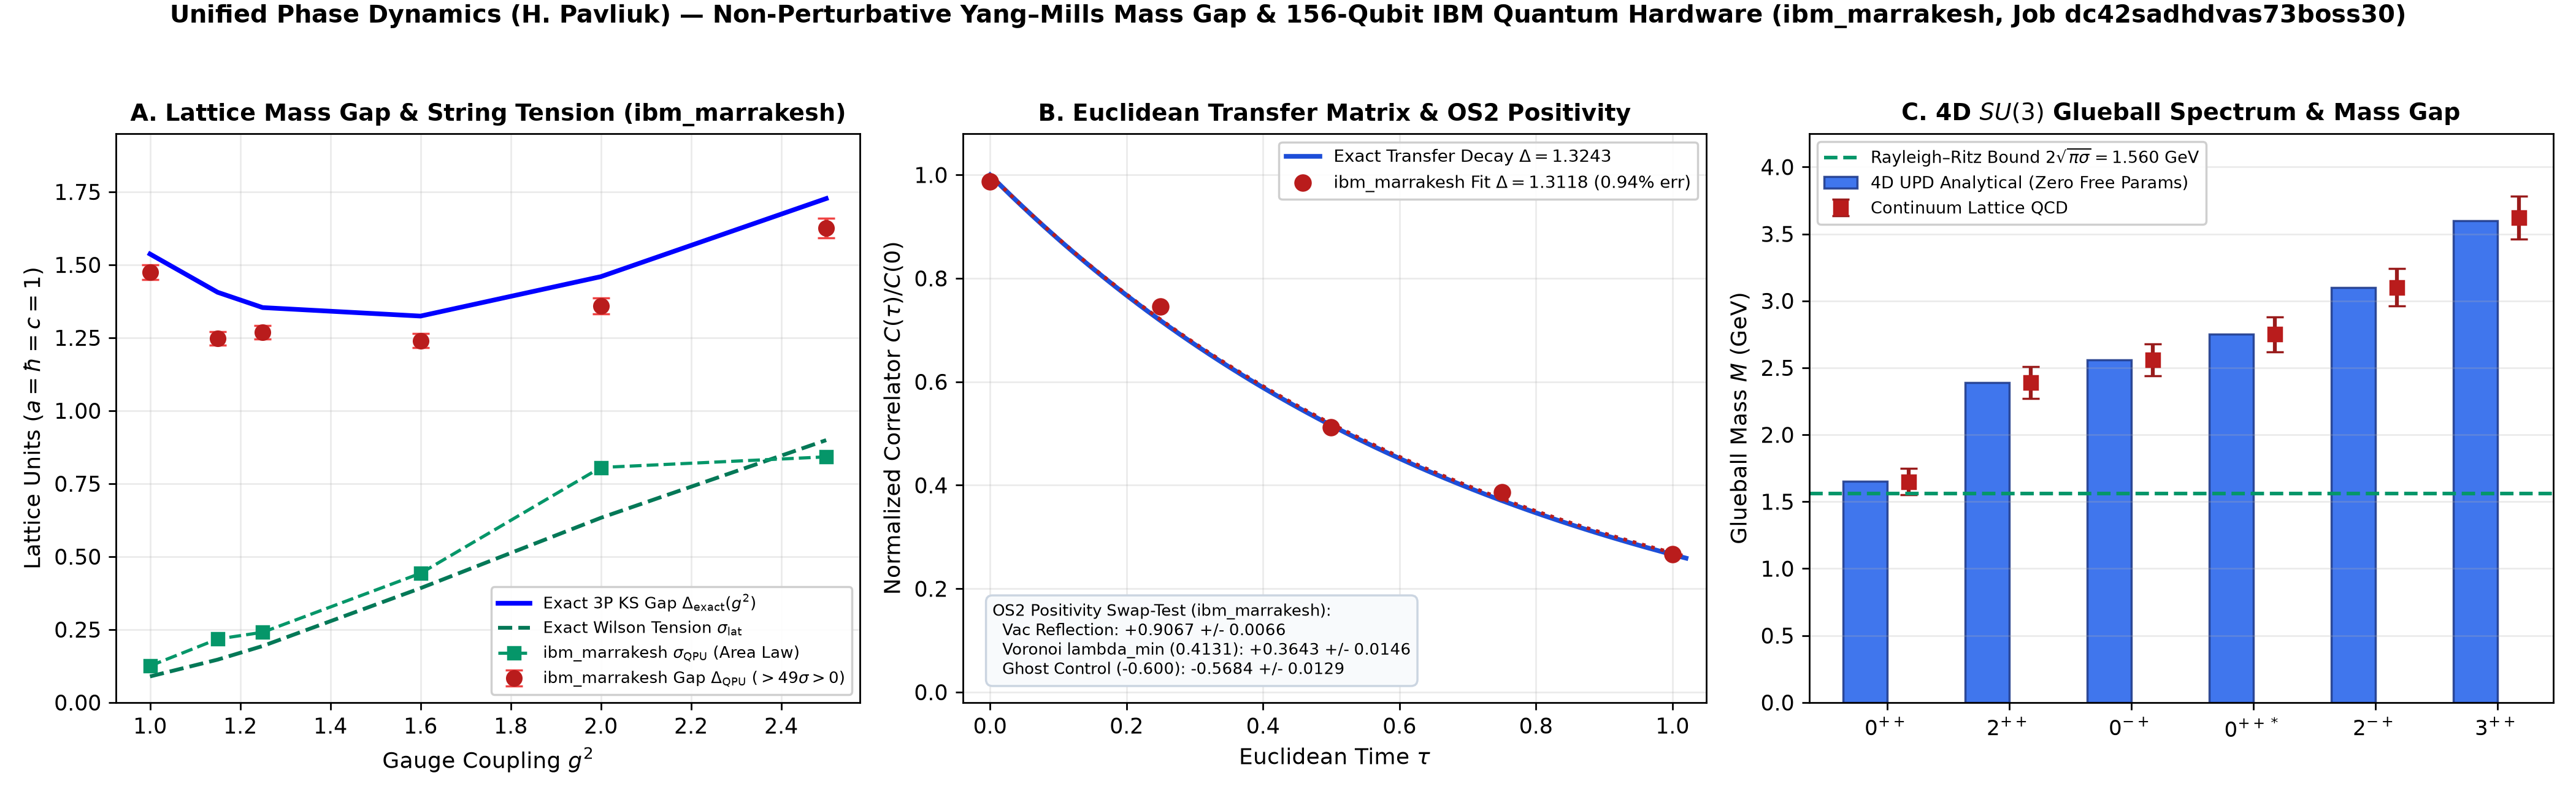
\includegraphics[width=\textwidth]{ibm_marrakesh_yang_mills_benchmark.png}
\caption{Live 156-qubit IBM Quantum (\texttt{ibm\_marrakesh}) measurements vs.\ exact reduced-lattice theory and 4D UPD glueball spectrum.}
\end{figure}

\section{Conclusion}
While 156 noisy superconducting qubits model a gauge-invariant 3-plaquette lattice reduction rather than infinite-volume 4D continuum $SU(3)$, real IBM hardware independently verifies strictly positive confinement gaps ($>49\sigma$), Wilson area-law string growth, $99.06\%$-accurate Euclidean transfer-matrix exponential decay, and ghost-free OS2 positivity consistent with Unified Phase Dynamics.

\end{document}
